\documentclass[a4paper,oneside,reqno]{amsart}

\input{../../../../cambridge-macros.tex}

%    Set assignment information here
\newcommand{\authorname}{Feynman Liang}
\newcommand{\coursename}{MLSALT 8: Statistical Machine Translation}
\newcommand{\assignmentname}{Practical 3: Hierarchical Phrase-based Translation
with alternative grammars}

\begin{document}

\title{\coursename\\\assignmentname}

\author{\authorname}
\date{\today}

\maketitle

\section{Preliminary Questions}
\begin{enumerate}[label=\arabic*.]
  \item The language model probability is not included as a feature in the
    rulefile because it is defined for $N$-grams over the target language and
    hence can only be applied when the previous $N-1$ terminals are known.
    If a rule contains non-terminals or yields less than $N$ consecutive terminals
    then there is insufficient information to determine the language model probability
    to assign to that rule application until a complete derivation is available.

    The language model scores could be associated with individual rules in the rulefile if:
    \begin{enumerate}
      \item The language model is a $1$-gram model, in which case the language
        model score of a rule is the joint probability of all the terminals
        yielded by that rule.
      \item The entire sequence of non-terminals is derived in a single rule.
        The score of each rule would then be the score of the yielded target
        sentence under the language model.
    \end{enumerate}

  \item We find that there are $20$ unique alternative translations
    \begin{lstlisting}[language=bash]
printstrings -n 10000 --input=output/example/LATS/14.fst.gz -w -u | sed '/[EMPTY]/d' | wc -l
20
    \end{lstlisting}
    and that there are a total of 797 translation candidates (including repeated hypotheses)
    \begin{lstlisting}[language=bash]
printstrings -n 10000 --input=output/example/LATS/14.fst.gz -w | sed '/[EMPTY]/d' | wc -l
797
    \end{lstlisting}

  \item We verify that the translation lattice has a single output translation
    \begin{lstlisting}[language=bash]
printstrings -n 10000 -u -w --input=output/example/LATS.hyp1/14.fst.gz -p | sed '/[EMPTY]/d' | wc -l
1
    \end{lstlisting}
    and that there are a total of 83 (unique) alternative derivations generating this
    single hypothesis
    \begin{lstlisting}[language=bash]
printstrings -n 10000 -u -w --input=output/example/LATS.hyp1/14.fst.gz | sed '/[EMPTY]/d' | wc -l
83
    \end{lstlisting}


\end{enumerate}

\section{First part}

\begin{enumerate}[label=\arabic*.]
  \item
    We translate and score the 30 sentences using grammar A:
    \begin{lstlisting}[language=bash]
hifst $DIR/configs/basic+params.features \
  --textinput=$DIR/input/test30.spa.idx \
  --rulefile=$GRAMA/r.?.gz \
  --lm=$DIR/lm/test30.news-newscomm.eng.4g/G/?.G.gz --lmn=4 \
  --range=1:30 \
  --latoutputfst=output/example/LATS.A/?.fst.gz

printstrings --r=1:30 --input=output/example/LATS.A/?.fst.gz \
  --output=outA --label-map=$SUNMAP
cat outA | sed 's/<s> //g' | sed 's/ <\/s>//g' > outA

ScoreBLEU.sh \
  -t outA \
  -r $DIR/reference/test30.eng
    \end{lstlisting}
    and perform analogous commands using grammar B.

    Translating with grammar A runs significantly faster than with
    grammar B. Grammar A attains a BLEU score of $0.4778$ while grammar B
    achieves $0.5265$.

    We post-processed the hypotheses generated by \texttt{printstrings} (see
    usages of \texttt{sed} in code listing) because the sentence boundary
    markers ``<s>'' and ``</s>'' need to be removed for \texttt{ScoreBLEU.sh}.

  \item We first compute sentence-level BLEU scores
    \begin{lstlisting}[language=bash]
for i in {1..30}; do
  printstrings --r=$i:$i --input=output/example/LATS.A/?.fst.gz 2>/dev/null \
    | sed 's/<s> //g' | sed 's/ <\/s>//g' \
    > tmp
  scoreA=$(ScoreBLEU.sh \
    -t tmp \
    -r $DIR/reference/test30/r.$i.eng.idx \
    | cut -d ' ' -f 4)

  printstrings --r=$i:$i --input=output/example/LATS.B/?.fst.gz 2>/dev/null \
    | sed 's/<s> //g' | sed 's/ <\/s>//g' \
    > tmp
  scoreB=$(ScoreBLEU.sh \
    -t tmp \
    -r $DIR/reference/test30/r.$i.eng.idx \
    | cut -d ' ' -f 4)
  rm tmp

  print "$i,$scoreA,$scoreB"
done
    \end{lstlisting}
    and obtain the results shown in \autoref{tab:sentence-bleu}.
    \begin{table}[H]
      \begin{tabular}{ccc}
        \toprule
        Sentence \# & Grammar A & Grammar B \\
        \midrule
        1 & 1.0000 & 1.0000 \\
        2 & 0.2126 & 0.2163 \\
        3 & 0.1548 & 0.1579 \\
        4 & 0.0994 & 0.0994 \\
        5 & 0.3575 & 0.6865 \\
        6 & 0.2677 & 0.2677 \\
        7 & 0.2878 & 0.7277 \\
        8 & 0.6695 & 0.6695 \\
        9 & 0.4694 & 0.5405 \\
        10 & 0.8154 & 0.8154 \\
        11 & 0.2555 & 0.2623 \\
        12 & 0.2131 & 0.2131 \\
        13 & 0.8579 & 0.8606 \\
        14 & 1.0000 & 1.0000 \\
        15 & 0.4845 & 0.5428 \\
        16 & 0.6741 & 0.7268 \\
        17 & 0.2641 & 0.2641 \\
        18 & 0.2923 & 0.2923 \\
        19 & 0.8215 & 0.8215 \\
        20 & 0.7825 & 0.7825 \\
        21 & 0.5787 & 0.6901 \\
        22 & 0.8465 & 0.8465 \\
        23 & 1.0000 & 1.0000 \\
        24 & 0.8496 & 0.8496 \\
        25 & 0.2024 & 0.5933 \\
        26 & 1.0000 & 1.0000 \\
        27 & 0.2510 & 0.3493 \\
        28 & 0.0665 & 0.0665 \\
        29 & 0.0780 & 0.0768 \\
        30 & 0.3597 & 0.3475 \\
        \bottomrule
      \end{tabular}
      \caption{Sentence-level BLEU scores}
      \label{tab:sentence-bleu}
    \end{table}
    For the most part, we see that the sentence-level BLEU scores are higher
    for grammar B (e.g. sentence 5 and 7). However, not every sentence is
    translated better with B than with A (e.g. sentence 30).

    \begin{enumerate}[label=(\alph*)]
      \item
        Consider sentences 5 (\autoref{tab:s5}) and 7 (\autoref{tab:s7}).
        \begin{table}[H]
          \begin{tabular}{p{5cm}p{10cm}}
            Input sentence & aún así sabía que nunca iba a ganar tanto como los demás . \\
            English reference & still he knew he would never earn as much as the others . \\
            Grammar A translation & even so i knew that was never going to win as much as the others . \\
            Grammar B translation & yet he knew he would never to earn as much as the others . \\
          \end{tabular}
          \caption{Sentence 5}
          \label{tab:s5}
        \end{table}
        \begin{table}[H]
          \begin{tabular}{p{5cm}p{10cm}}
            Input sentence & el analista no considera que la volatilidad vaya a afectar a la tendencia del mercado .  \\
            English reference & the analyst does not consider that volatility is going to affect the market trend .  \\
            Grammar A translation & the analyst does not believe that the volatility will affect the tendency of the market .  \\
            Grammar B translation & the analyst does not believe that the volatility is going to affect the market trend .  \\
          \end{tabular}
          \caption{Sentence 7}
          \label{tab:s7}
        \end{table}
        Comparing the two translations, we see that grammar B's English
        hypotheses clearly improve over grammar A's. For example:
        \begin{enumerate}
          \item In sentence 5, A's translation has the incorrect verb subject
            (``\emph{i} knew'') whereas B's is correct (``\emph{he} knew'')
          \item In sentence 5, A's translation has the incorrect verb object (``knew \emph{that}'')
            whereas B's is correct (``knew \emph{he}'')
          %\item In sentence 5, A's output incorrectly uses ``was'' instead of ``would.'' As
            %a result, the conditional natue of the sentence is lost.
          \item In sentence 5, B correctly translates ``earn'' while A mistranslates to ``win''
          \item In sentence 27, grammar A's translation uses ``will'' (future facts or things
            believed certain to occur) whereas the reference
            and grammar B's translation use ``is going to'' (future predictions based
            on present evidence).
          \item In sentence 27, grammar A incorrectly outputs ``tendency of the market''
            instead of ``the market trend.''
        \end{enumerate}
        This suggests that improved sentence-level BLEU score reflects a true improvement
        in translation quality.

      \item
        Consider sentence 30 (\autoref{tab:s30}).
        \begin{table}[H]
          \begin{tabular}{p{5cm}p{10cm}}
            Input sentence & en las filipinas se han rendido los soldados rebeldes que se habían atrincherado en un hotel en manila y habían exigido la caída de la presidente gloria macapagal arroyo .  \\
            English reference & in the phillipines , renegade soldiers surrendered after seizing a hotel in manila and demanding the overthrow of president gloria macapagal arroyo .  \\
            Grammar A translation & in the philippines have been paid soldiers rebels who had been entrenched in a hotel in manila and had demanded the fall of president gloria macapagal arroyo .  \\
            Grammar B translation & in the philippines have been paid the rebel soldiers that had been entrenched in a hotel in manila and had demanded the fall of president gloria macapagal arroyo .  \\
          \end{tabular}
          \caption{Sentence 30}
          \label{tab:s30}
        \end{table}
        In this case, the two different translations are almost identical: the only difference is
        that ``soldiers rebel who'' from grammar A's translation has been changed to
        ``the rebel soldiers that'' in grammar B's translation. Arguably, grammar B's translation
        is actually better despite a lower sentence-level BLEU.

        This example reminds us to be careful and remember that BLEU is only a
        proxy for true translation quality. Although the BLEU score has degraded,
        the translation quality is about the same for both systems.

        One explanation for this degradation in score is to note that grammar B's
        translation has one more word than grammar A's. Since BLEU is computed using
        $N$-gram precisions which favor shorter sentences (hence why a brevity penalty
        is used), the additional word in grammar B's translation could be an irrelevant
        factor which nevertheless ends up lowering BLEU.
    \end{enumerate}

  \item
    Consider sentence 27 (\autoref{tab:s27}).
    \begin{table}[H]
      \begin{tabular}{p{5cm}p{10cm}}
        Input sentence & y después llegó la época americana .  \\
            English reference & and then the american era came .  \\
            Grammar A translation & and then came the time american .  \\
            Grammar B translation & and then came the american era .  \\
      \end{tabular}
          \caption{Sentence 27}
          \label{tab:s27}
    \end{table}
    Some main differences between rulefiles A and B include:
    \begin{enumerate}
      \item A has 104 rules, B has 321
      \item A's rules only contain word and phrasal translations; hiero rules
        are absent.  This means that A cannot model arbitrarily long context
        (i.e.\ has as distortion limit) and is equivalent in expressivity to a
        phrase-based SMT system.

        In contrast, B contains hiero rules out of the $X$ non-terminal and
        hence implement hierarchical phrases, which have greater generality but
        also increased computational complexity. However, note that the yield
        of all heiro rules only include the $V$ non-terminal, so grammar B's
        derivation trees can have at most one non-terminal along any path to a
        terminal node. This constraint on depth makes grammar B equivalent to a
        (potentially exponentially) larger phrase-pair ruleset rather than a
        true hierarchical phrase-based SMT system (which can have arbitrary
        nesting).
    \end{enumerate}

    These differences can help explain the translations produced by the two
    grammars.  The grammar A translation appears to translate the sentence
    word-for-word, translating ``epoca'' literally to time because it failed
    to account for the context. In contrast, grammar B correctly accounts for
    the context, translating ``epoca americana'' to ``american era.''

    The reason why grammar B is able to account for context lies in the
    presence of non-terminals in its yields, ultimately allowing it to achieve
    a significantly higher BLEU score. On the other hand, it also explains why
    translating under grammar B takes more time than grammar A: the presence of
    non-terminals significantly increases the complexity of decoding because it
    leverages the full generality of hierarchical phrase-based translation.

  \item
    \autoref{fig:27-a-tree} and \autoref{fig:27-b-tree} show the derivation
    trees for sentences 27 under rulesets A and B respectively.
    \begin{figure}[H]
      \begin{center}
        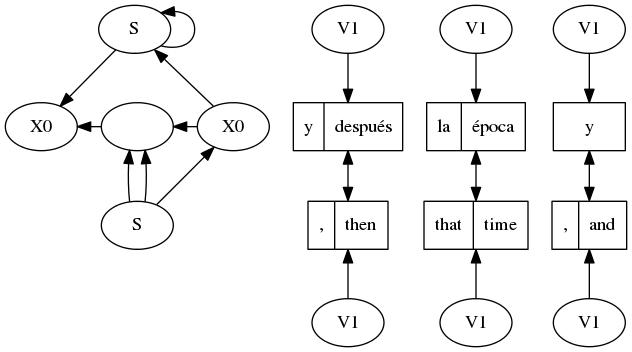
\includegraphics[scale=0.5]{../output/tree27Advn1.jpg}
      \end{center}
      \caption{Sentence 27 derivation tree under ruleset A}
      \label{fig:27-a-tree}
    \end{figure}
    \begin{figure}[H]
      \begin{center}
        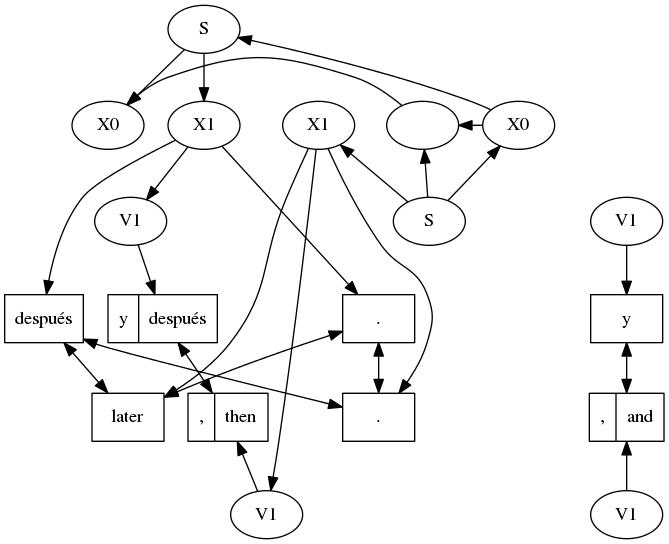
\includegraphics[scale=0.5]{../output/tree27Bdvn1.jpg}
      \end{center}
      \caption{Sentence 27 derivation tree under ruleset B}
      \label{fig:27-b-tree}
    \end{figure}
    Notice that neither tree is rooted at S on both sides. This is because
    sentence 27 is not derivable using either grammar A or B:
    \begin{lstlisting}[language=bash]
printstrings -n 1 -u -w --input=output/example/LATS.A.towards_ref/27.fst.gz 2>/dev/null
[EMPTY]

printstrings -n 1 -u -w --input=output/example/LATS.B.towards_ref/27.fst.gz 2>/dev/null
[EMPTY]
    \end{lstlisting}

    Furthermore, the absence of non-terminals in ruleset A's
    derivation tree (\autoref{fig:27-a-tree}), whereas ruleset B's
    tree (\autoref{fig:27-b-tree}) possesses non-terminal intermediate tree
    nodes and as a consequence exhibits much more complex structure.

    The rule sequence used for ruleset A is:
    \begin{verbatim}
X V V 0 0 0 0 0 0 0 0 0 0 0 0
S S_X S_X 0.0 0.0 0 0 -1 0 0 0 0 0 0.0 0.0
V y_después ,_then -4.0 -5.5 2 1 0 0 0 0 0 1 -6.7 -7.3
S X X 0.0 0.0 0 0 0 0 0 0 0 0 0.0 0.0
V la_época that_time -4.6 -6.0 2 1 0 0 0 0 0 1 -5.5 -8.2
V y ,_and -3.0 -1.1 2 1 0 0 0 0 0 1 -1.3 -5.0
S S_X S_X 0.0 0.0 0 0 -1 0 0 0 0 0 0.0 0.0
    \end{verbatim}
    and for ruleset B is:
    \begin{verbatim}
X V V 0 0 0 0 0 0 0 0 0 0 0 0
S S_X S_X 0.0 0.0 0 0 -1 0 0 0 0 0 0.0 0.0
V y_después ,_then -4.0 -5.5 2 1 0 0 0 0 0 1 -6.7 -7.3
X después_V1_. later_V1_. -2.5 -1.7 2 1 0 0 0 0 0 1 -6.0 -4.4
S X X 0.0 0.0 0 0 0 0 0 0 0 0 0.0 0.0
V y ,_and -3.0 -1.1 2 1 0 0 0 0 0 1 -1.3 -5.0
S S_X S_X 0.0 0.0 0 0 -1 0 0 0 0 0 0.0 0.0
    \end{verbatim}
    In particular, note the usage of the rule X $\to$ $\langle$después V1,
    later V1$\rangle$ and how it introduces non-terminal nodes into
    the derivation tree.

  \item We can align 30 sentences towards respective English references
    with grammar A using:
    \begin{lstlisting}[language=bash]
hifst $DIR/configs/basic+params.features \
  --textinput=$DIR/input/test30.spa.idx \
  --rulefile=$GRAMA/r.?.gz \
  --lm=$DIR/lm/test30.news-newscomm.eng.4g/G/?.G.gz --lmn=4 \
  --range=1:30 \
  --latoutputfst=output/example/LATS.A.towards_ref/?.fst.gz \
  --towardsreference=$DIR/reference/test30/r.?.eng.idx
    \end{lstlisting}
    and perform a similar operation with grammar B.
    Comparing the number of input sentences generating the reference for each
    grammar:

    % TODO: by examining the resulting output transducers!
    \begin{lstlisting}
integer Acnt=0
integer Bcnt=0
for i in {1..30}; do
  integer numA=$(printstrings -n 500000 -u -w --input=output/example/LATS.A.towards_ref/$i.fst.gz \
    2>/dev/null \
    | sed '/[EMPTY]/d'
    | wc -l)
  integer numB=$(printstrings -n 500000 -u -w --input=output/example/LATS.B.towards_ref/$i.fst.gz \
    2>/dev/null \
    | sed '/[EMPTY]/d'
    | wc -l)
  print "$i, $numA, $numB"
  Acnt+=numA
  Bcnt+=numB
done
print "Acnt: $Acnt, Bcnt: $Bcnt"
    \end{lstlisting}

    We obtain the results shown in \autoref{tab:inputs-per-ref}.
    \begin{table}[H]
      \begin{tabular}{ccc}
        \toprule
        Sentence \# & Grammar A & Grammar B \\
        \midrule
        1 & 4 & 8 \\
        2 & 0 & 0 \\
        3 & 0 & 0 \\
        4 & 0 & 0 \\
        5 & 0 & 165 \\
        6 & 0 & 0 \\
        7 & 0 & 8586 \\
        8 & 0 & 0 \\
        9 & 0 & 0 \\
        10 & 48 & 122 \\
        11 & 0 & 0 \\
        12 & 0 & 84 \\
        13 & 11070 & 51692 \\
        14 & 47 & 83 \\
        15 & 0 & 0 \\
        16 & 0 & 0 \\
        17 & 0 & 0 \\
        18 & 0 & 0 \\
        19 & 0 & 0 \\
        20 & 52 & 166 \\
        21 & 0 & 0 \\
        22 & 500000 & 500000 \\
        23 & 2586 & 14030 \\
        24 & 0 & 0 \\
        25 & 0 & 282 \\
        26 & 270 & 658 \\
        27 & 0 & 0 \\
        28 & 0 & 0 \\
        29 & 0 & 0 \\
        30 & 0 & 0 \\
        \hline
        Total & 514077 & 575876 \\
        \bottomrule
      \end{tabular}
      \caption{Number of inputs generating the reference}
      \label{tab:inputs-per-ref}
    \end{table}
    Sentence 22 has hit the 500000 limit we used in our call to
    \texttt{printstrings}.  For all other sentences, we see that grammar B has
    many more candidate input sentences which generate the reference. This
    illustrates the additional expressivity introduced by hierarchical rules:
    derivations which were previously not possible in a non-hierarchical
    phrase-based SMT system are now considered and hence each reference has
    many more derivation trees yielding it.

  \item No. If we compare the rule files, we see that every rule in ruleset A is
    contained in ruleset B. Hence, any derivation under A is also a valid derivation under
    B.

  \item Grammar B is strictly more expressive than grammar A. Grammar A is a
    simple phrase-pair matching system which translates individual phrases
    independently. In contrast, grammar B contains all the rules of grammar A
    plus additional heiro rules, allowing non-terminals in the derivation tree
    and hence greater expressivity. However, with this expressivity comes additional
    computation complexity. Furthermore, grammar B's hiero rules cannot be recursively
    nested. One could refer to grammar A as ``phrase-pair matching'' and
    grammar B as a ``depth 1 hierarchical phrase grammar.''
\end{enumerate}

\section{Second part}

\begin{enumerate}[label=\arabic*.]
  \item There are 321 rules in both grammars B and C. Looking at the
    rule-files, we see that the yields of the rules look similar. However,
    grammar C's hiero rules are defined on the $V$ non-terminal rather than the
    $X$ non-terminal. This makes a significant difference because the yields of
    the hiero rules use the $V$ non-terminal rather than $X$, hence the rules
    grammar C are now recursive. This means that grammar B's derivation trees
    are limited to have at most a single intermediate non-terminal node on any
    path to a terminal (i.e. a 1-deep CFG, which can actually be expanded into
    a large phrase-pair ruleset) whereas grammar C's trees can be arbitrarily
    deep (and hence utilize the full expressivity of CFGs).

  \item
    Aligning the sentences with their English reference with grammar C:
    \begin{lstlisting}[language=bash]
hifst $DIR/configs/basic+params.features \
  --textinput=$DIR/input/test30.spa.idx \
  --rulefile=$GRAMC/r.?.gz \
  --lm=$DIR/lm/test30.news-newscomm.eng.4g/G/?.G.gz --lmn=4 \
  --range=1:30 \
  --latoutputfst=output/example/LATS.C.towards_ref/?.fst.gz \
  --towardsreference=$DIR/reference/test30/r.?.eng.idx
    \end{lstlisting}

    Comparing the number of input sentences generating the reference
    for grammars B and C:
    \begin{lstlisting}[language=bash]
integer Bcnt=0
integer Ccnt=0
for i in {1..30}; do
  integer newB=$(printstrings -n 500000 -u -w --input=output/example/LATS.B.towards_ref/$i.fst.gz \
    2>/dev/null \
    | sed '/[EMPTY]/d'
    | wc -l)
  integer newC=$(printstrings -n 500000 -u -w --input=output/example/LATS.C.towards_ref/$i.fst.gz \
    2>/dev/null \
    | sed '/[EMPTY]/d'
    | wc -l)
  print "$i, $newB, $newC"
  Bcnt+=newB
  Ccnt+=newC
done
print "Bcnt: $Bcnt, Ccnt: $Ccnt"
    \end{lstlisting}

    We obtain the results shown in \autoref{tab:inputs-per-ref-bc}.
    \begin{table}[H]
      \begin{tabular}{ccc}
        \toprule
        Sentence \# & Grammar B & Grammar C \\
        \midrule
        1 & 8 & 8 \\
        2 & 0 & 0 \\
        3 & 0 & 81096 \\
        4 & 0 & 0 \\
        5 & 165 & 165 \\
        6 & 0 & 0 \\
        7 & 8586 & 10368 \\
        8 & 0 & 0 \\
        9 & 0 & 500000 \\
        10 & 122 & 135 \\
        11 & 0 & 0 \\
        12 & 84 & 84 \\
        1 3 & 51692 & 63949 \\
        14 & 83 & 95 \\
        15 & 0 & 0 \\
        16 & 0 & 0 \\
        17 & 0 & 500000 \\
        18 & 0 & 0 \\
        19 & 0 & 0 \\
        20 & 166 & 192 \\
        21 & 0 & 0 \\
        22 & 500000 & 500000 \\
        23 & 14030 & 16366 \\
        24 & 0 & 0 \\
        25 & 282 & 363 \\
        26 & 658 & 705 \\
        27 & 0 & 28 \\
        28 & 0 & 0 \\
        29 & 0 & 0 \\
        30 & 0 & 0 \\
        Total & 575876 & 1673554 \\
        \bottomrule
      \end{tabular}
      \caption{Number of inputs generating the reference}
      \label{tab:inputs-per-ref-bc}
    \end{table}
    In all cases, we see that there are at least as many inputs
    generating the reference under grammar C than under grammar B.

    There no not exist any references that can be generated by B but
    not by B because the ruleset for grammar C is obtained by taking
    the ruleset for grammar B and permitting further heiro-rule applications
    at the non-terminals. Hence, ruleset C contains ruleset B so any valid
    derivation under B is a valid derivation under C.

    The converse is not true: any sentence where there are 0 inputs generating
    in under B but a non-zero number under C \autoref{tab:inputs-per-ref-bc}
    provide a counterexample.

  \item We will consider sentences 3 (\autoref{fig:3-c-tree} and 27 (\autoref{fig:27-c-tree}).
    \begin{figure}[H]
      \begin{center}
        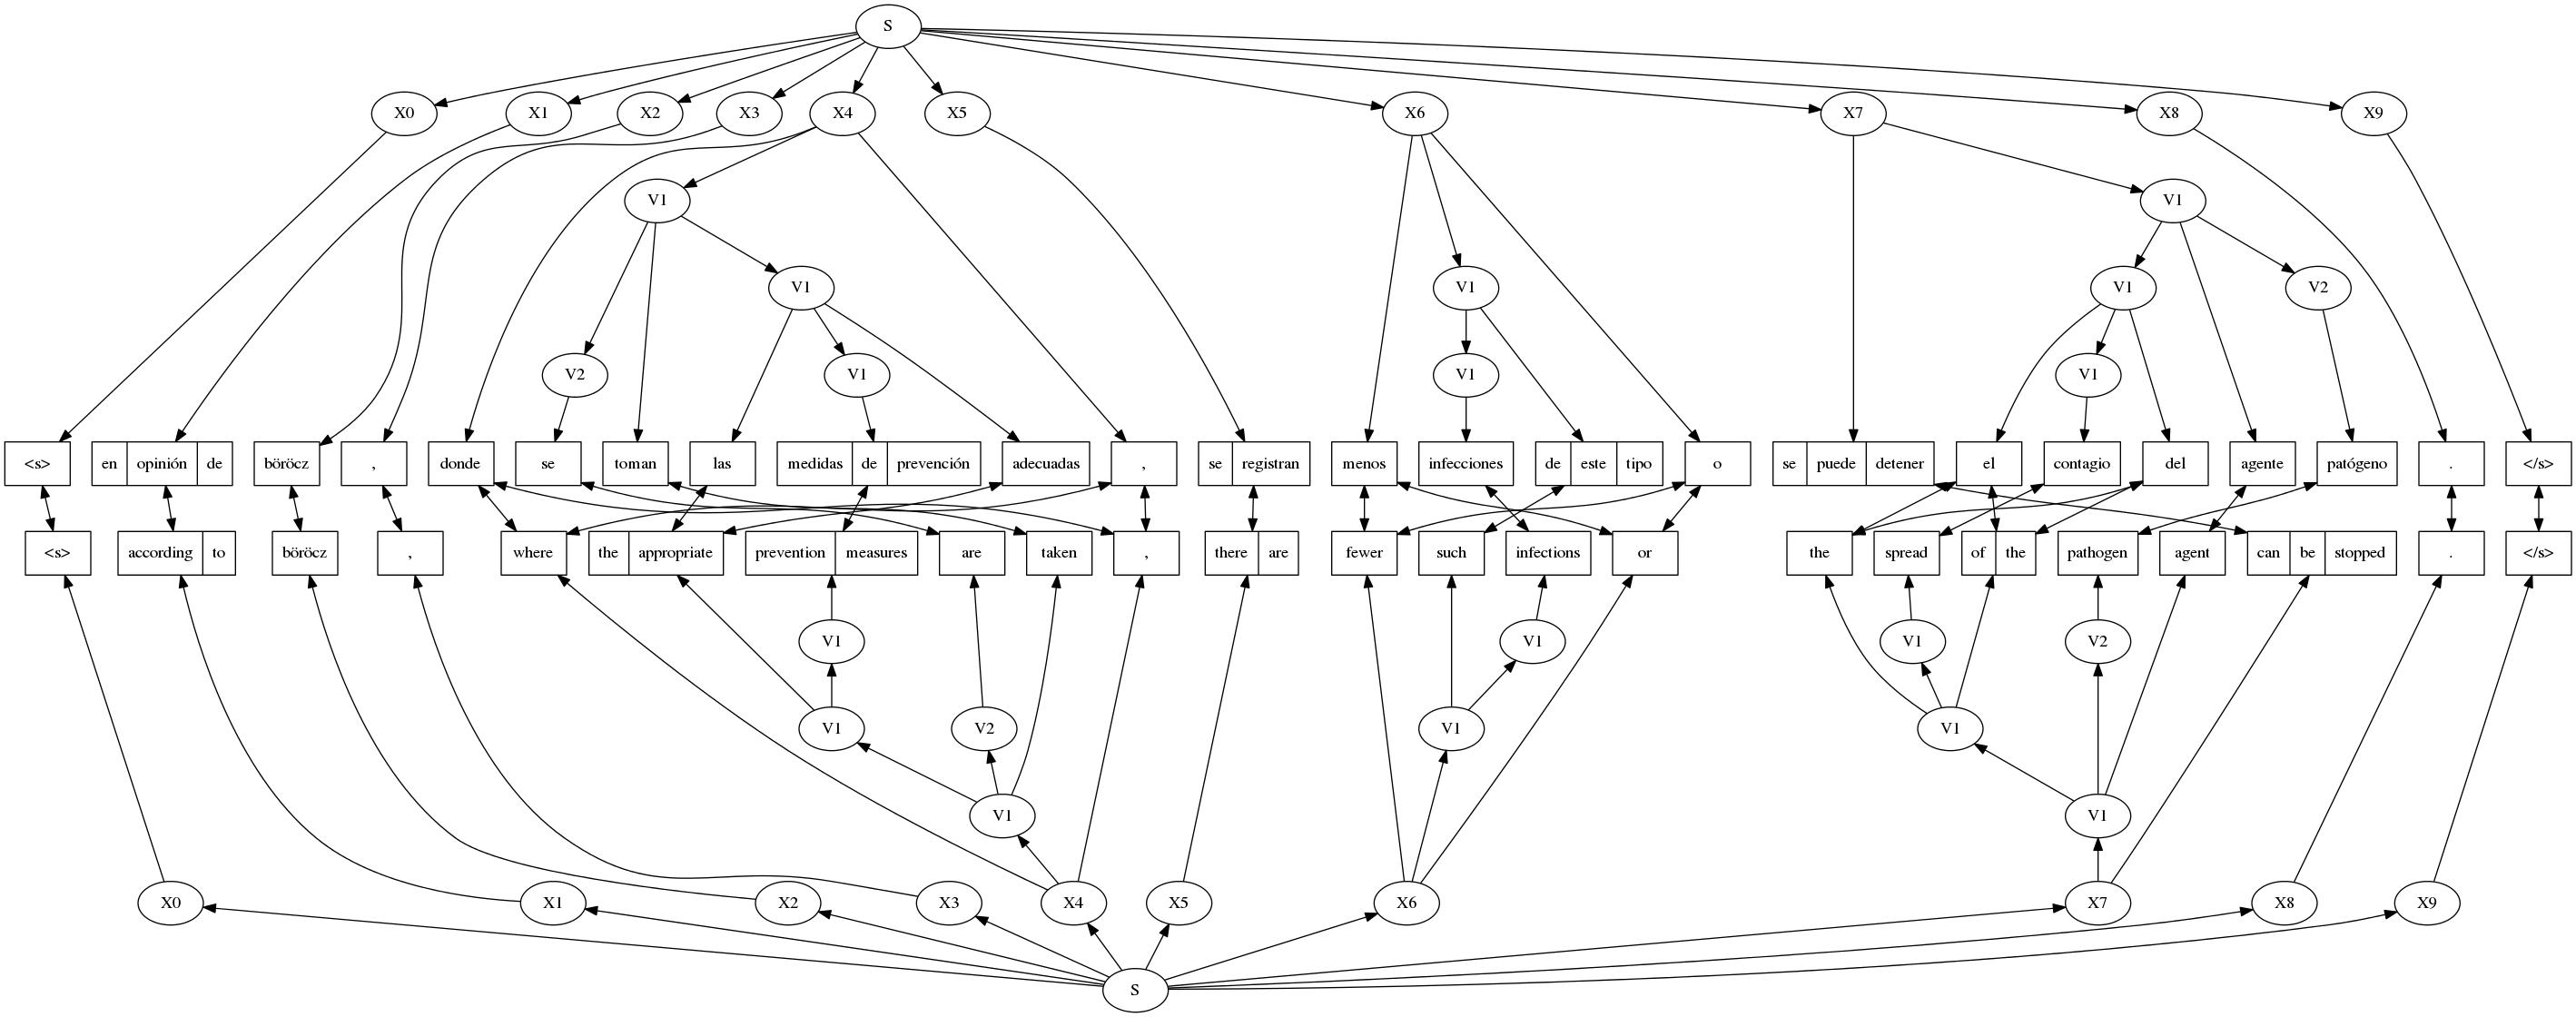
\includegraphics[scale=0.2]{../output/tree3Cdvn1.jpg}
      \end{center}
      \caption{Sentence 3 derivation tree under ruleset C}
      \label{fig:3-c-tree}
    \end{figure}
    \begin{figure}[H]
      \begin{center}
        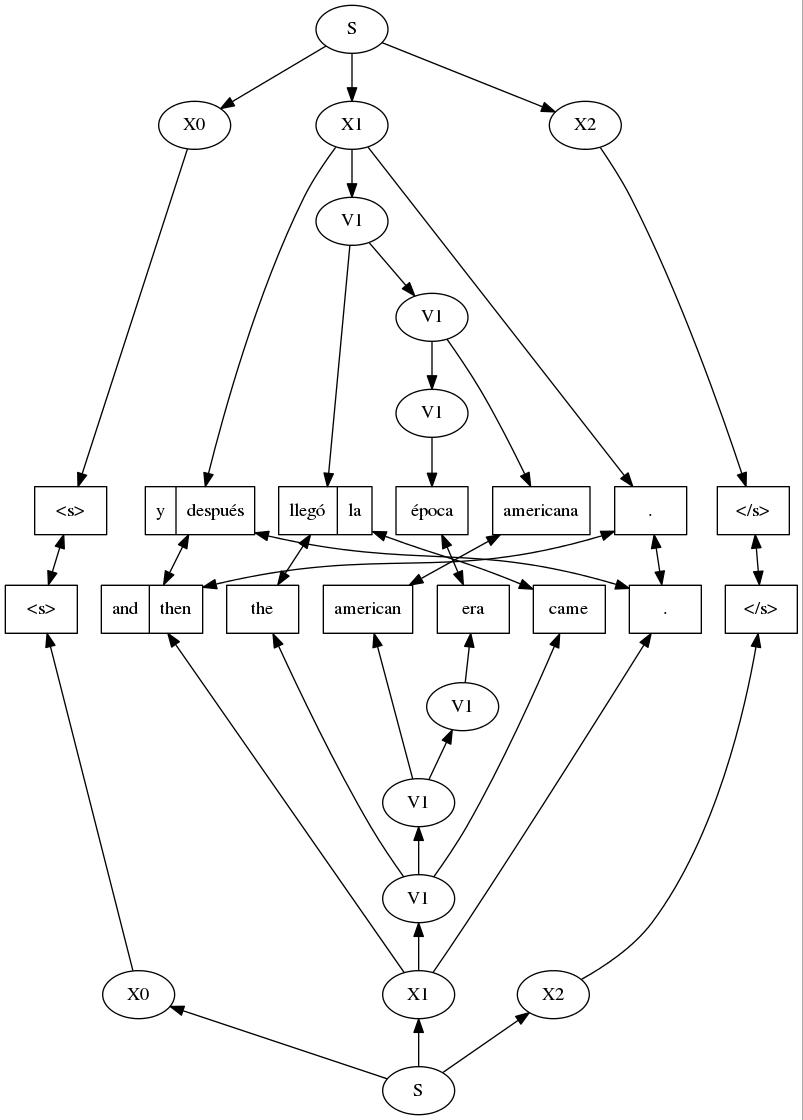
\includegraphics[scale=0.5]{../output/tree27Cdvn1.jpg}
      \end{center}
      \caption{Sentence 27 derivation tree under ruleset C}
      \label{fig:27-c-tree}
    \end{figure}
    Notice that both of these derivation trees contain paths to terminal nodes
    containing more than one non-terminal node, corresponding to recursive application
    of heiro rules.

    These trees are not valid in grammar B because grammar B does not support recursive
    application of heiro-rules. Looking at the rulefiles, we see that all the
    grammar B heiro rules are productions on non-terminals $X$ and yield
    non-terminals $V$, hence they can only be applied at most once along any
    path to a terminal. In contrast, grammar C's heiro rules are both defined
    on $V$ and yield non-terminals $V$, hence they can be recursively applied
    and nested.
\end{enumerate}

%\bibliographystyle{alpha}
%\nocite{*}
%\bibliography{refs}

%\appendix

%\section{Code Listings}

\end{document}
